\documentclass{article}


\usepackage{../../austin137}
\usepackage{../../local}
\usehyperstuff

\begin{document}

%%%%%%%%%%%%%%%%%%%%%%%%%%%%%%%%%%%%%%%%%%%%%%%%%%%%%%%%%%%%%%%%%%%%%%%%%%%%%%%%
\addcopyright
\begin{center}
{\bf \large Physics W89 - Introduction to Mathematical Physics - Summer 2023}\\\medskip
{\bf \large Problem Set - Module 02 - What's Your Vector, Victor?} \\\medskip
{\emph{Last Update: \today}}
\end{center}


\dphline\bigskip
%%%%%%%%%%%%%%%%%%%%%%%%%%%%%%%%%%%%%%%%%%%%%%%%%%%%%%%%%%%%%%%%%%%%%%%%%%%%%%%%
\section*{Problem 2.1 - The Dual Vector Space}
\relevid{Introduction to Vectors and Vector Spaces}

%%%%%%%%%%%%%%%%%%%%%
\paragraph{}
In lecture we expanded our notion of what a vector can be by defining a vector space as a set of vectors that are closed under \heavydef{vector addition} and \heavydef{scalar multiplication},
where vector addition and scalar multiplication were defined via a set of eight vector space axioms.  
We saw that the familiar ``arrows in 3D space'' vectors that were used all throughout intro physics were indeed vectors (they
provided the template for defining a vector!) and we also saw that things like the shape of waves on a string could act as vectors.  In this problem we explore another
important set of vectors called the \heavydef{dual vector space}.

\paragraph{}
In short, a \heavydef{dual vector} is a machine that \emph{eats a vector and returns a scalar in a linear fashion}.  That is, a dual vector $\dual{\alpha}$ is a
\heavydef{linear function} from a vector space $V$ to the real (or complex) numbers, $\dual{\alpha}:V\to\mathbb{R}$ (or $\mathbb{C}$),
	\begin{equation}
		\dual{\alpha}(a\vec{v}_{1}+b\vec{v}_{2}) = a\,\dual{\alpha}(\vec{v}_{1})+ b\,\dual{\alpha}(\vec{v}_{2}).
	\label{duallinear}
	\end{equation}
Note that we have a notational decoration for dual vectors (an underline) just like we have a notational decoration for vector (the ``arrow hat'').

\paragraph{}
Given a vector space $V$, the \heavydef{dual space} $V^{*}$ is abstractly\footnote{Oh, boy!  I'll bet you all \emph{love} seeing \emph{this} word pop up!} 
defined as the set of all linear functions from the vector space to the scalars.  In this problem we will take our scalars to be the real numbers.  Another way of expressing this definition is,
	\begin{equation*}
		V^{*} \equiv \setdef{\dual{\alpha}:V\to\mathbb{R}}{\! \dual{\alpha}\textrm{ is linear}}.
	\end{equation*}

For this problem the vector space $V$ will be $\mathbb{R}^{3}$, the three-dimensional vectors (like force, velocity, displacement, etc.), which we will write in
component form as a column of three numbers, $\vec{v} = \smthreevect{v_{x}}{v_{y}}{v_{z}}$.  

\phline
%%%%%%%%%%%%%%%%%%%%%
\paragraph{}
First let's explore what these dual vectors are and aren't by looking at some examples of what is and isn't in $V^{*}$. 


%%%%%%%%%%%%%%%%%%%%%
\paragraph{(a)}
Show that the function that picks out the $x$-component of a vector $\dual{\beta}{}_{x}(\vec{v}) \equiv v_{x}$ is an element of $V^{*}$.  Then argue that the same holds
for the function that picks out the $y$-component and $z$-component of a vector.\\
\note{When I ask you to ``show'' something, you are basically providing a short proof.  In this case, to show that $\dual{\beta}{}_{x}$ is an element of $V^{*}$, you need
to test whether it satisfies the defining property of linearity, Eq.~\ref{duallinear}.  When I ask you to ``argue'' something, it doesn't need to be a formal or detailed proof.  It
should be something like a sentence or two explaining why the result follows.  This will usually be a reference to a previous proof or an appeal to symmetry.}

\begin{solution}
    To show that $\beta_x$ is an element of the dual vector space, we simply have to show that $\beta_x$ maps to $\mathbb R$ and is also linear. The mapping part is easy: when expressed in component form, $v_x$ is a real number that represents the projection of the vector $\vec v$ onto the $x$-axis. To show that it's linear, suppose we have two vectors $\vec v, \vec w$:
    \begin{align*}
        \beta_x(\vec v + \vec w) &= \beta_x((v_x + w_x)\hat x + (v_y + w_y)\hat y + (v_z + w_z) \hat z) = v_x + w_x\\
        \beta_x(\vec v) + \beta_x(\vec w) &= v_x + w_x
    \end{align*}
    And since these two are the same value, then the operation is linear, and hence is an element of $V^*$.
\end{solution}


%%%%%%%%%%%%%%%%%%%%%
\paragraph{(b)}
Show that the ``length'' function $\delta(\vec{v}) \equiv \abs{\vec{v}} = \sqrt{v_{x}^{2}+v_{y}^{2}+v_{z}^{2}}$ is \emph{not} an element of $V^{*}$ by coming up
with an explicit example of the failure of linearity, Eq.~\ref{duallinear}.

\begin{solution}
    Suppose we have the two vectors $\hat i$ and $\hat j$, represented in their component form as $\hat i = (1, 0, 0)$ and $\hat j = (0, 1, 0)$ \footnote{I use row vectors here just for the sake of writing these in-line, writing column vectors here would be painful to read.}. Now we check for linearity:
    \begin{align*}
        \delta(\hat i + \hat j) &= \delta((1, 1, 0)) = \sqrt{2}\\
        \delta(\hat i) + \delta(\hat j) &= 1 + 1 = 2
    \end{align*}
    And since $\sqrt{2} \neq 2$, then this operation is \textit{not} linear, hence it is not an element of $V^*$.
\end{solution}

%%%%%%%%%%%%%%%%%%%%%
\paragraph{}
We may define the vector addition and scalar multiplication of dual vectors via the action of the resulting map on vectors,
	\begin{alignat*}{2}
		\textrm{Vector Addition:} &\quad& (\dual{\alpha}+\dual{\beta})(\vec{v}) &\equiv \dual{\alpha}(\vec{v}) + \dual{\beta}(\vec{v}),\\
		\textrm{Scalar Multiplication:} && (a\dual{\alpha})(\vec{v}) &\equiv a\big(\dual{\alpha}(\vec{v})\big).	
	\end{alignat*}
Define $\dual{\zeta}$ to be the ``zero dual vector,'' which spits out 0 no matter what vector is fed to it, $\dual{\zeta}(\vec{v}) = 0\ \forall\ \vec{v}$.

\paragraph{(c)}
Show that vector addition and scalar multiplication of dual vectors satisfy the eight axioms for a vector space.\\
\note{This is the \ul{only} time (including exams) that I'll explicitly ask you to check these eight axioms, but it's good to go through it once.  
An example of showing the commutativity of vector addition (the first axiom) is given as a supplement.
Don't overthink this part!  A lot of the axioms will be pretty trivially satisfied.}

\begin{solution}
    Running through the list:
    \begin{itemize}
        \item \textbf{Commutativity under addition:} $\alpha(\vec v) + \alpha(\vec w) = \alpha(\vec w) + \alpha(\vec v)$. This is satisfied becuase addition of real numbers is commutative.
        \item \textbf{Associativity under addition:} $\alpha(\vec v) + (\alpha(\vec w) + \alpha(\vec u)) = (\alpha(\vec v) + \alpha(\vec w)) + \alpha(\vec u)$. Just like the previous one, this is satisfied because addition of real numbers is also associative.
        \item \textbf{Zero Vector:} By definition we have introduced $\zeta(\vec v)$ as the ``zero vector" in our case, since $\alpha(\vec v) + \zeta(\vec v) = \alpha(\vec v)$, which is the definition of a zero vector.
        \item \textbf{Additive Inverse:} Define a dual vector $\beta(\vec v) = -\alpha(\vec v)$. Then, $\beta(\vec v)$ is the additive inverse of $\alpha(\vec v)$. One could also check that $\beta \in V^*$, either by brute force or simply noting that multiplication by a negative sign is a linear operation.
        \item \textbf{Associativity under scalar multiplication:} We use the second principle:
        \[ (ab\alpha)(\vec v) = ab(\alpha(\vec v)) = ba(\alpha(\vec v)) = (ba\alpha)(\vec v)\]
        as required. Here we used the definition of scalar multiplication to bring $ab$ out of the parentheses, used the fact that multiplication is associative, then used the definition of scalar multiplication again to bring $ba$ back into the parentheses.
        \item \textbf{Multiplicative Identity:} $1 \cdot \alpha(\vec v) = \alpha(\vec v)$. This is obvious since $\alpha(\vec v) \in \mathbb R$.
        \item \textbf{Distributive with scalar sums:} $(c_1 + c_2)\alpha(v) = c_1\alpha(v) + c_2\alpha(v)$. This property holds because $\alpha(v) \in \mathbb R$, and multiplication is distributive over scalar sums.
        \item \textbf{Distributive under vector sums:} $c(\alpha(\vec v) + \alpha(\vec w)) = c\alpha(\vec v) + c\alpha(\vec w)$. Again, because $\alpha(\vec v), \alpha(\vec w) \in \mathbb R$, these operations are also distributive over scalar sums so this principle holds as well.
    \end{itemize}
\end{solution}

%%%%%%%%%%%%%%%%%%%%%
\paragraph{}
Finally, for $V^{*}$ to be a vector space we need it to be \heavydef{closed} under addition and scalar multiplication.  That is, we
need to show that the sum of two dual vectors is itself a dual vector and the scaling of a dual vector is a dual vector.

\paragraph{(d)}		\extrapart
Show that $V^{*}$ is closed under vector addition and scalar multiplication and is thus a vector space!


%%%%%%%%%%%%%%%%%%%%%
\paragraph{(e)}
Use the results from (a) and (d) to argue that the function that picks out a specific linear combination of components, 
$\dual{\beta}(\vec{v}) = b_{x}v_{x} + b_{y}v_{y} 
+ b_{z}v_{z}$ is an element of $V^{*}$, where $b_{x}, b_{y}, b_{z}$ are all real constants.

\begin{solution}
    We can express $\dual{\beta}(\vec v) = b_x\beta_x(\vec v) + b_y\beta_y(\vec v) + b_z\beta_z(\vec v)$ and from part d) we know that $V^*$ is closed under vector addition and scalar multiplication, so hence they are also closed under any combination of addition and scalar multiplication. Thus, $\dual{\beta}(\vec v)$, which we've just expressed as a linear combination of three other dual vectors $\beta_x, \beta_y, \beta_z$, it must follow that $\dual{\beta}(\vec v) \in V^*$.
\end{solution}


\paragraph{}
\noindent\emph{Commentary: We won't prove it here, but in fact \emph{all} dual vectors of $\mathbb{R}^{3}$ can be interpreted in this way!  Once we introduce matrices, we will be able to write 
these dual vectors as \heavydef{row vectors}, at which point the action of the dual vector simply becomes matrix multiplication.}


\bigskip
\dphline
\pagebreak
%%%%%%%%%%%%%%%%%%%%%%%%%%%%%%%%%%%%%%%%%%%%%%%%%%%%%%%%%%%%%%%%%%%%%%%%%%%%%%%%
\section*{Problem 2.2 - Vector Identities in 3D}
\relevid{3D Vectors and Index Notation}

%%%%%%%%%%%%%%%%%%%%%
\paragraph{}

In lecture we introduced the Kronecker delta $\delta_{ij}$ and the Levi-Civita symbol $\epsilon_{ijk}$ which let us express the dot product and cross product of
vectors in our usual three-dimensional space in terms of components.  You should use Einstein summation convention (any repeated index is summed over)
throughout this problem.

%%%%%%%%%%%%%%%%%%%%%
\paragraph{(a)}
Derive the vector triple product identity $\vec{A}\times(\vec{B}\times\vec{C}) = (\vec{A}\bcdot\vec{C})\vec{B} - (\vec{A}\bcdot\vec{B})\vec{C}$
using the Kronecker delta and Levi-Civita symbol.  Carefully explain and/or justify each step you take (e.g. ``by the antisymmetry of $\epsilon_{ijk}$...'').
\spoilers{Start with the left-hand side.  Since both sides are vectors, we really want to show the component-version of the identity,
$\big(\vec{A}\times(\vec{B}\times\vec{C})\big)_{i} = (\vec{A}\bcdot\vec{C})B_{i} - (\vec{A}\bcdot\vec{B})C_{i}$.}

\begin{solution}
    Just follow the index notation:
    \begin{align*}
        \vec A \times (\vec B \times \vec C) &= \epsilon^{ijk}A_j\epsilon^{kmn} B_mC_n \\
        &= \epsilon^{ijk}\epsilon^{kmn} A_j B_m C_n\\
        &= \epsilon^{kij}\epsilon^{kmn} A_j B_m C_n\\
        &= (\delta_{im} \delta_{jn} - \delta_{in}\delta_{jm}) A_j B_m C_n\\
        &= A_i B_i C_j - A_j B_j C_i\\
        &= B_i\underbrace{(A_j C_j)}_{\vec A \cdot \vec C} - C_i\underbrace{(A_j B_j)}_{\vec A \cdot \vec B}\\
        &= (\vec A \cdot \vec C)\vec B - (\vec A \cdot \vec B)\vec C
    \end{align*}
\end{solution}


%%%%%%%%%%%%%%%%%%%%%
\paragraph{(b)}		\extrapart
Using index notation, show \heavydef{Lagrange's identity},
	\begin{equation*}
		(\vec{A}\times\vec{B})\bcdot(\vec{A}\times\vec{B}) = (\vec{A}\bcdot\vec{A})(\vec{B}\bcdot\vec{B}) - (\vec{A}\bcdot\vec{B})^{2}.
	\end{equation*}


\phline
%%%%%%%%%%%%%%%%%%%%%
\paragraph{}
We can treat the nabla/del symbol from vector calculus in components as: $\vec{\nabla} \mapsto \partial_{i}\equiv \pdiff{}{x_{i}}$.
Using this, the gradient, divergence, and curl can be expressed in index notation:
	\begin{alignat*}{3}
		\textrm{Gradient:}&\qquad& 
			(\vec{\nabla}f)_{i} &= \partial_{i}f, \\
		\textrm{Divergence:}&\qquad&
			\vec{\nabla}\bcdot\vec{v} &= \delta_{ij}\partial_{i}v_{j}, \\
		\textrm{Curl:}&\qquad&
			(\vec{\nabla}\times\vec{v})_{i} &= \epsilon_{ijk}\partial_{j}v_{k}. 
	\end{alignat*}

\paragraph{(c)}		\extrapart
Write out the \heavydef{Laplacian} of a scalar function $\nabla^{2}f = \vec{\nabla}\bcdot\vec{\nabla}f$ in index notation and then carry out the sum.



%%%%%%%%%%%%%%%%%%%%%
\paragraph{(d)}
Prove that the curl of the gradient is zero: $\vec{\nabla}\times(\vec{\nabla}f) = \vec{0}$.

\begin{solution}
    Writing this out in index notation, we have:
    \[ \curl (\nabla f) = \epsilon^{ijk} \partial_j (\partial k f) = \epsilon^{ijk}\partial_j \partial_k f = -\epsilon^{ikj}\partial_k \partial_j f\]
    Now, we use the fact that since partial derivatives can be swapped without consequence (known as Clairaut's theorem) to argue that these two values must be equal in quantity. As a result, we've come to the conclusion that $x = -x$, and hence the only solution to this is $x = 0$, so therefore:
    \[ \curl(\nabla f) = -\curl(\nabla f) \implies \curl(\nabla f) = 0\]
\end{solution}

%%%%%%%%%%%%%%%%%%%%%
\paragraph{(e)}
Prove that the curl of the curl is given by $\vec{\nabla}\times(\vec{\nabla}\times\vec{A}) = \vec{\nabla}(\vec{\nabla}\bcdot\vec{A}) - \nabla^{2}\vec{A}$.

\begin{solution}
    Again just carry out the index notation:

    \begin{align*}
        \curl(\curl \vec A) &= \epsilon^{ijk}\partial_j \epsilon^{kmn} \partial_m A_n\\
        &= \epsilon^{ijk}\epsilon^{kmn} \partial_j \partial_m A_n\\
        &= \epsilon^{kij}\epsilon^{kmn} \partial_j \partial_m A_n \\
        &= (\delta_{im}\delta_{jn} - \delta_{in}\delta_{jm}) \partial_j \partial_m A_n\\
        &= \underbrace{\partial_j \partial_i A_j}_{\partial_i(\partial_j A_j)} - \partial_j \partial_j A_i\\
        &= \nabla(\div \vec A) - \nabla^2 \vec A
    \end{align*}
\end{solution}

\pagebreak
%%%%%%%%%%%%%%%%%%%%%%%%%%%%%%%%%%%%%%%%%%%%%%%%%%%%%%%%%%%%%%%%%%%%%%%%%%%%%%%%
\section*{Problem 2.3 - Subspace Communication}
\relevid{Linear Independence and Span;  Bases}


%%%%%%%%%%%%%%%%%%%%%
\paragraph{}
A \heavydef{subset} of a vector space $W\subset V$ is any collection of objects from the vectors space.  In some cases the subset is itself a vector space, in which case we case the subset a
\heavydef{vector subspace}.  Since vector addition and scalar multiplication carry over from $V$ to $W$, to determine whether a subset is a subspace, we only need to check that it is 
closed under vector addition and scalar multiplication\footnote{See, for example, Problem 2.1(d).} - that is, we need to check that an arbitrary linear combination of elements of the subset is itself an 
element of the subset.  Note that \emph{by definition}, the span of a set of vectors $\{\vec{v}_{i}\in V\}$ is a subspace of $V$.  Also note that for a given vector space $V$, the full space 
$V$ and the subset $\{\vec{0}\}$ just containing the zero vector are always subspaces.  The zero subspace is zero-dimensional.

%%%%%%%%%%%%%%%%%%%%%
\paragraph{(a)}
Consider a vector space $V$ and a subset $W\subset V$.  Show or argue that if the zero vector is not part of a subset ($\vec{0}\notin W$) then $W$ \emph{can't} be a vector subspace.\\
\note{We say that the zero vector being a part of $W$ is a \emph{necessary} but \emph{not a sufficient} condition for $W$ to be a subspace.  That is, for $W$ to be a subspace it needs to
contain the zero vector but $W$ containing the zero vector isn't enough to claim $W$ is a subspace.}
\extrasubpart{Try to come up with an example of a subset $W$ that contains the
zero vector but is not a vector subspace of $V=\mathbb{R}^{2}$.} 

\begin{solution}
    We know that vector spaces are closed under vector addition and scalar multiplication. Now suppose $W$ is a vector subspace that doesn't contain the zero vector. Then, given a vector $\vec v \in W$, we know that $W$ is closed under scalar multiplication so $-\vec v \in W$ as well. $W$ must also be closed under vector addition meaning that $\vec v + (-\vec v) = \vec v - \vec v = \vec 0 \in W$. This is a contradition to our original statement, since we initially assumed that $\vec 0 \not \in W$. Therefore $\vec 0 \in W$ is a necessary condition for $W$ to be a vector subspace.
\end{solution}


\phline
%%%%%%%%%%%%%%%%%%%%%
\paragraph{}
Consider the collection of all polynomials (with real coefficients) of degree less than or equal to $N$ in the real variable $x$, which we may write as
	\begin{equation}
		P_{N} \equiv \Bigg\{\sum_{j=0}^{N} a_{j}x^{j}\ \Bigg|\ a_{j}\in\mathbb{R}\Bigg\}.
	\label{polynomials}
	\end{equation}
We can take as our starting point that the space of \emph{all} polynomials (with no upper limit on the degree) is a vector space.

%%%%%%%%%%%%%%%%%%%%%
\paragraph{(b)}
For each of the following subsets, state whether or not the set constitutes a vector space.  If so, suggest a convenient basis and give the dimension of the space.  
If not, explain or show why not.  You do not need to explicitly or rigorously \emph{prove} that your suggested basis is a basis, but you should \emph{argue}
that the elements of your basis are indeed linear independent and do in fact span the subset.
	\begin{itemize}
		\item The full set $P_{N}$ given by Eq.~\ref{polynomials}.

  \begin{solution}
      $P_N$ is a vector space, since addition of polynomials is done by adding the coefficients of terms of the same order, and since these coeffficients remain real then the resulting vector is also a part of $P_N$. Scalar multiplication is distributive across a polynomial (i.e. every coefficient is multiplied by that scalar), and since multiplication of real numbers is still a real number, the resulting polynomial is also in $P_N$. Thus, $P_N$ is a vector space.

      As for the basis, we can choose the list $\{1, x, x^2, \dots, x^n\}$ since any linear combination of these will create any polyonial we'd like.
  \end{solution}
		\item The subset of $P_{N}$ such that the leading coefficient of the polynomial is 1 (that is, the set such that $a_{N} = 1$).
  \begin{solution}
      This is not a vector space, since it's not closed under addition. Suppose we take two polynomials $p_n, p_m$. When adding $p_n + p_m$, the leading coefficient will now be 2, since both $p_n, p_m$ had leading coefficients of 1. But because this leading coefficient is not 1 it is not part of the vector space, hence this subset fails the definition of vector addition.
  \end{solution}
		\item The subset of $P_{N}$ such that the polynomials have the value 0 at $x=1$.

  \begin{solution}
      We can write every polynomial in this subset as $p_n = (x - 1) q_n$, where $q_n$ is the remaining part of the polynomial. Since there are no restrictions on $q_n$, these polynomials will also be closed under vector addition and scalar multiplication in the same way we proved part that the full set of $P_N$ is closed. Therefore, this is a vector space. 
	  
	  To show this more explicitly, suppose we have two polynomials $p_n, p_m$:
	  \[ p_m + p_n = (x - 1)q_m + (x-1) q_n = (x-1)(q_m + q_n)\]
	  and since the resulting polynomial has a root at $x = 1$, this is satisfied. As for scalar multiplication, 
	  a similar thing occurs: 
	  \[ c p_n = c(x - 1) q_n = (x-1)(cq_n)\] 
	  Again, giving us a polynomial which has a root at $x = 1$, hence this is also satisfied. 

	  For the basis, we can just take the basis we used for $P_N$ and slap an $x - 1$ term everywhere: $\{x - 1, x(x - 1), x^2(x - 1), \dots, (x -1)x^{n-1}\}$. When forming linear combinations of these vectors, we can then just
	  factor the $x - 1$ out leaving us with the basis $\{1, x, x^2, \dots, x^{n-1}\}$, which we already know from the first subpart is able to generate any polynomial $q_n$, meaning that the full polynomial we generate would be $p_n = (x - 1)q_n$ as desired. 
  \end{solution}
		\item \emph{Supplementary Part (Not for Credit):} The subset of $P_{N}$ such that the polynomials have the value 1 at $x=0$.
	\end{itemize}

	\begin{solution}
		This subset has $a_N = 1$, but this would also not be closed under vector addition since if we add two 
		polynomials from this set we'd get $a_N = 2$, which is not part of this subset. Therefore, this is 
		not a valid subspace.
	\end{solution}

\bigskip
\pagebreak
\bigskip
%%%%%%%%%%%%%%%%%%%%%%%%%%%%%%%%%%%%%%%%%%%%%%%%%%%%%%%%%%%%%%%%%%%%%%%%%%%%%%%%
\section*{Problem 2.4 - A Wave on a String}
\relevid{Bases; The Inner Product}

%%%%%%%%%%%%%%%%%%%%%
\paragraph{}
Next let's look at our ``waves on a string'' vector space - the space of continuous real functions $f(x)$ between $x=0$ and $x=L$ with $f(0) = f(L) = 0$ (the string is fixed at zero
at the endpoints).  We can abstractly refer to one of our shapes as a vector $\vec{g}$ in this space or ``in components'' as a function $g(x)$.  Consider the set of vectors
$\{\hat{f}_{n}\}$,
	\begin{equation*}
		\hat{f}_{n} \doteq f_{n}(x) = \sqrtfsm{2}{L}\sin\left(\fracsm{n\pi x}{L}\right),	\qquad n \in \mathbb{N}
	\end{equation*}
with $n$ a positive integer ($n=1,2,3,\cdots$).
We define the inner product between two vectors $\vec{g}$ and $\vec{h}$ in this space of functions as
	\begin{equation}
		\vec{g}\bcdot\vec{h} \equiv \int_{0}^{L} g(x)h(x)\,dx.
	\label{stringscalar}
	\end{equation}

%%%%%%%%%%%%%%%%%%%%%
\paragraph{(a)}
Show that the set of vectors $\{\hat{f}_{n}\}$ is an orthonormal set.  That is, show $\hat{f}_{n}\bcdot\hat{f}_{m} = \delta_{nm}$.
\extrasubpart{Show that this implies the set $\{\vec{f}_{n}\}$ is linearly independent.}
\note{This set also turns out to span our vector space (this is called \heavydef{Fourier's theorem}) and thus it serves as an orthonormal basis!}

\begin{solution}
    To show orthornality we just take the inner product:

    \begin{align*}
        \hat f_n \cdot \hat f_m &= \frac{2}{L} \int_0^L \sin\left( \frac{n \pi x}{L}\right) \sin\left(\frac{m \pi x}{L}\right)
    \end{align*}
    We can perform a $u$-substitution $u = \frac{\pi x}{L} \implies du = \frac{\pi}{L} dx$, which gives:

    \[ \frac{2}{\pi} \int_0^\pi \sin(nu) \sin(mu) du\]

    Then, we can perform a bit of exponential tricks, and skipping some algebra that I don't want to type, we get:
    \[ -\frac{1}{2\pi}\left[\int_0^\pi \left( e^{i(n + m)u } - e^{i(n - m) u} - e^{-i(n - m) u} + e^{-i(n + m)u}\right) dx\right]\]

    When $n = m$, this integral simplifies to:
    \begin{align*}
        -\frac{1}{2\pi} \int_0^\pi e^{i 2nu} - e^0  - e^0 + e^{-i(2nu)} du &= -\frac{1}{2\pi} \left[\frac{e^{2inu}}{2in} - 2u - \frac{e^{-2inu}}{2in}\right]_0^\pi\\
        &= -\frac{1}{2\pi} \left[\frac{e^{2in \pi}}{2in} - 2\pi - \frac{e^{-2i n \pi}}{2in}\right]\\
        &= -\frac{1}{2\pi} \left[\frac{\sin(2n\pi)}{n} - 2\pi\right]\\
        &= 1
    \end{align*}
    In the last step here we use $\sin(2n \pi) = 0$. Now for $n \neq m$, we can proceed with the earlier integral which will give us:
    \[ -\frac{1}{2\pi} \left[ \frac{e^{i(n + m)u}}{i(n + m)} - \frac{e^{i(n - m)u}}{i(n - m)} - \frac{e^{-i(n - m) u }}{-i(n - m)} + \frac{e^{-i(n +m)u}}{-i(n + m)}\right]_0^\pi\]
    When evaluating the bounds, we find that when $u = 0$ we have: 
    \[ \frac{1}{n + m} - \frac{1}{n - m} + \frac{1}{n - m} - \frac{1}{n + m} = 0\]
    Therefore, we only have $u = \pi$ terms. After a bit of simplification after plugging $u = \pi$ in, we get:
    \[
        -\frac{1}{\pi}\left[ \frac{1}{n + m}\underbrace{\frac{e^{i(n + m)\pi} - e^{-i(n + m)\pi}}{2i}}_{\sin((n + m) \pi)} - \frac{1}{n - m} \underbrace{\frac{e^{i (n - m)\pi} - e^{-i(n - m) \pi}}{2i}}_{\sin((n - m)\pi)}\right]
    \]
    And since we know that $\sin(k\pi) = 0$ when $k$ is an integer, then this whole term in the square brackets goes to zero, so hence this expression gives 0 for $n \neq m$. Therefore, we find that this inner product return 1 when $n = m$ and 0 when $n \neq m$, which is exactly what $\delta_{mn}$ does as well. Therefore: 
    \[ \hat f_n \cdot \hat f_m = \delta_{mn}\]
\end{solution}

%%%%%%%%%%%%%%%%%%%%%
\paragraph{(b)}		\extrapart
Argue that the given inner product does indeed satisfy the three defining features of the inner product (conjugate symmetry, linearity in the second term, and positive-definiteness).


\phline
%%%%%%%%%%%%%%%%%%%%%
\paragraph{}
Since we have an orthonormal basis, we can expand any vector $\vec{g}$ in our vector space (any ``shape on our guitar string'') as
	\begin{equation}
		\vec{g} = \sum_{n=1}^{\infty} c_{n}\hat{f}_{n},
	\label{expansion}
	\end{equation}
where $c_{n}$ are a set of real coefficients, the ``components'' of the function.

\paragraph{(c)}
Show that we can find the coefficients $c_{n}$ in Eq.~\ref{expansion} by taking the inner product $\hat{f}_{n}\bcdot\vec{g}$.\\
\note{This is an extremely important proof and result!}
\spoilers{Be careful with indices.  We are already using the index $n$ in the expression $\hat{f}_{n}\bcdot\vec{g}$.  When you substitute in
equation Eq.~\ref{expansion} for $\vec{g}$, you will need to use a different summation index (e.g. $m$).}

\begin{solution}
    We write $\vec g = \sum c_n \hat f_n$. Then taking the inner product:
    \begin{align*}
        \hat f_n \cdot \vec g &= \hat f_n \cdot \sum c_m \hat f_m \\
        &= \sum c_m \hat f_n \cdot \hat f_m\\
        &= \sum c_m \delta_{mn}\\
        &= c_n
    \end{align*}
    as desired.
\end{solution}
%%%%%%%%%%%%%%%%%%%%%
\paragraph{}
Suppose we pluck the string so that the shape is described by the following ``triangle''  function,
	\begin{equation}
		\vec{g} \doteq g(x) = 
			\begin{cases}
				x, & 0\leq x \leq L/2,\\
				(L-x), & L/2 \leq x \leq L.
			\end{cases}
	\label{pluck}
	\end{equation}
%%%%%%%%%%%%%%%%%%%%%
\paragraph{(d)}		  
Find the components $c_{n}$.  Try finding $c_{n}$ for $n$ odd first, and then find $c_{n}$ for $n$ even.
\spoilers{Remember our result from part (c)!  Exploit symmetry and think before you integrate! One of your expressions should be zero.}

\begin{solution}
    Taking the inner product, we have: 
    \[ \hat f_n \cdot \vec g = \int_0^{L/2} \sqrt{\frac 2L} \sin\left( \frac{n \pi x}{L}\right) x dx + \int_{L/2}^L \sqrt{\frac 2L } \sin \left( \frac{n \pi x}{L}\right) (L - x) dx \]
    Now we do this by cases, starting out with $n$ odd. I threw this into mathematica, and it gave me: %fix this
    \[ \sqrt{\frac 2L} \left[ -\frac{L^2(n \pi \cos(n \pi /2) - 2 \sin(n \pi /2))}{2n^2\pi^2} - \frac{L^2(n \pi \cos(n \pi /2) + 2\sin(n \pi /2) - 2 \sin (n\pi))}{2n^2 \pi^2}\right] \]
    Here, there are a lot of simplifications we can make. First, we note that $\sin(n \pi) = 0$ and $\cos(n \pi/2) = 0$ for all $n$. As a result, this actually causes the first and second term to be equal. Further, $\sin(n \pi/2)$ alternates between $\pm 1$, at every odd number, starting with $+1$ when $n = 1$. Therefore this simplifies to
    \[c_{2n + 1} = \sqrt{\frac 2L} 2 \cdot \frac{2L^2(-1)^n}{2(2n+1)^2\pi^2} = \sqrt{\frac2L} \frac{2L^2(-1)^n}{(2n+1)^2\pi^2}\]
    which is the formula for all the odd coefficients. For even $n$, we find that the function is antisymmetric about $x = L/2$ (I found this out while playing around in desmos and also through office hours), so therefore the first integral actually equals the negative of the second integral, hence the sum of the two integrals gives us zero. Therefore the even coefficients, written as $c_{2n}$, are all zero. As a final result, we get: 
    \begin{align*}
        c_{2n} &= 0\\
        c_{2n + 1} &= \sqrt{\frac 2L} 2 \cdot \frac{2L^2(-1)^n}{2(2n+1)^2\pi^2} = \sqrt{\frac2L} \frac{2L^2(-1)^n}{(2n+1)^2\pi^2}
    \end{align*}
    as the coefficients for even and odd $n$.
\end{solution}

%%%%%%%%%%%%%%%%%%%%%
\paragraph{}
If this string were stretched taut on a guitar, then releasing the string from the pluck described in Eq.~\ref{pluck} makes a sound.  The value $c_{1}$ tells you about
the amplitude of the \heavydef{fundamental frequency} of the sound and the other values of $c_{n}$ can be interpreted as the amplitudes of each of the \heavydef{harmonics}.  The total energy 
produced by the sound wave is proportional to the magnitude-squared of the vector $\vec{g}$, and the energy contained in any harmonic is proportional (with the same proportionality constant)
to the magnitude-equared of the coefficient $c_{n}$.  Letting $\eta$ be the proportionality constant,
	\begin{equation*}
		E_{\textrm{wave}} = \eta\,\vec{g}\bcdot\vec{g};	\qquad	
		E_{\textrm{n-th harmonic}} = \eta\abs{c_{n}}^{2}.
	\end{equation*}
Therefore, the fraction of energy contained in a harmonic is given by $\abs{c_{n}}^{2}/\abs{\vec{g}}^{2}$.

\paragraph{(e)} 
Given the triangle wave $\vec{g}$ from the previous part, what fraction of energy is in the fundamental ($n=1$) frequency?  The first harmonic ($n=2$)?
\spoilers{You already found $c_{1}$ and $c_{2}$ in part (d)!}

\begin{solution}
    First we find $|\vec g|^2 = \vec g \cdot \vec g$, which gives: 
    \[ \int_0^{L/2} x^2 dx + \int_{L/2}^L (L - x)^2 dx = \frac{L^3}{24} + \frac{L^3}{24} = \frac{L^3}{12}\]
    Then, for $n = 1$, we have 
    \[ c_1 = \sqrt{\frac 2L} \frac{2L^2}{\pi^2} \implies |c_1|^2 = \frac{8L^3}{\pi^4}\]
    Therefore, the fraction contained in the first harmonic is: 
    \[ \frac{|c_1|^2}{|\vec g|^2} = \frac{\frac{8L^3}{\pi^4}}{\frac{L^3}{12}} = \frac{96}{\pi^4}\]
    For the first harmonic, we note that $c_2 = 0$, so immediately we get that $|c_2|^2/|\vec g|^2 = 0$, and hence the fraction of energy in the first harmonic is zero.
\end{solution}


%%%%%%%%%%%%%%%%%%%%%
\paragraph{(f)}		\extrapart
\ul{Physics refresher/reminder!}
Suppose the string had a lineal mass density of $\mu$ and was under tension $T$.  What is the wave speed?  What is the fundamental frequency $\omega_{1}$?  
The frequency of the $n$-th harmonic $\omega_{n}$?


%%%%%%%%%%%%%%%%%%%%%
\paragraph{(g)}
Let $L=1$ and graph\footnote{Go-go-gadget Python/Mathematica/WolframAlpha/MatLab/etc.} the triangle function $g(x)$ and the 
partial sums
	\begin{equation*}
		\sum_{n=1}^{n_{\textrm{max}}} c_{n}f_{n}(x),
	\end{equation*}
of the expansion for $n_{\textrm{max}} = 3, 5, 10, 50$ to see how the series converges to the true function $g(x)$.

\begin{solution}
    I threw this into python and got:
    \begin{center}
        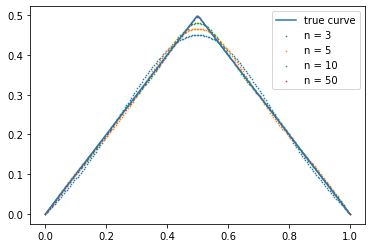
\includegraphics[scale=0.8]{image.png}
    \end{center}
    This plot also clearly shows that the more terms we introduce, the closer we get to the true triangle wave. In fact, $n_{\text{max}} = 50$ is such a good approximation that the dots are barely visible in this picture. 
\end{solution}


\bigskip
\dphline
\pagebreak
%%%%%%%%%%%%%%%%%%%%%%%%%%%%%%%%%%%%%%%%%%%%%%%%%%%%%%%%%%%%%%%%%%%%%%%%%%%%%%%%
\section*{Problem 2.5 - A Block Sliding Down an Incline}
\relevid{The Inner Product; The Gram-Schmidt Procedure}

%%%%%%%%%%%%%%%%%%%%%
\paragraph{}
You thought you'd never see these first-semester physics ``block slides down a slope'' problems again?  Consider a triangular piece of plane whose vertices are positions 
$\vec{V}_{1} = \smthreevect{0}{0}{2.4}, \vec{V}_{2} = \smthreevect{0}{4}{0}, \vec{V}_{3} = \smthreevect{3}{0}{0}$.  These vectors are written with respect to the unit vectors 
$\hat{x}, \hat{y},\hat{z}$, with $\hat{z}$ being the ``vertically up'' direction.  Consider the three ``edge vectors'' which form the edges of the plane,
	\begin{equation*}
		\vec{A} = \vec{V}_{2}-\vec{V}_{1} = \smthreevect{0}{4}{-2.4},	\qquad 
		\vec{B} = \vec{V}_{3}-\vec{V}_{2} = \smthreevect{3}{-4}{0},		\qquad
		\vec{C} = \vec{V}_{1}-\vec{V}_{3} = \smthreevect{-3}{0}{2.4},
	\end{equation*}

%%%%%%%%%%%%%%%%%%%%%
\paragraph{(a)}
Explicitly show that $\{\vec{A}, \vec{B}, \vec{C}\}$ is \emph{not} a linearly independent set and does \emph{nor} span $\mathbb{R}^{3}$.
\spoilers{This means explicitly constructing a linear combination of two of the vectors to create the third to show linear dependence and showing that there is a vector
in $\mathbb{R}^{3}$ that cannot be expressed as a linear combination of the three vectors.}

\begin{solution}
    We note that $C = -(\vec A + \vec B)$, therefore $\{\vec A \vec B \vec C\}$ is not a linearly independent set. To show that it doesn't span $\mathbb R^3$, we first set up the system of equations:
    \begin{align}
        3b -3c &= x\\
        4a - 4b &= y\\
        -2.4a + 2.4c &= z
    \end{align}
    where $\smthreevect{x}{y}{z}$ is the vector we want to find. A bit of poking around in WolframAlpha finds that the vector $\smthreevect{0}{3}{7}$ cannot be created, since there are no solutions for $a, b, c$ when we plug in $x = 0, y = 3, z = 7$ into our system.
\end{solution}


\phline
%%%%%%%%%%%%%%%%%%%%%
\paragraph{}
The span of the edge vectors creates a plane that passes through the origin, $P \equiv \textrm{Span}(\vec{A},\vec{B},\vec{C})$.  
We want to build an orthonormal basis to describe objects moving around on our plane.
Since these three vectors are linearly dependent, we may ignore one of them when building a basis. 

\paragraph{(b)}
Use the Gram-Schmidt procedure on the ordered pair $\{\vec{B},\vec{A}\}$ to form an orthonormal basis $\{\hat{e}_{1},\hat{e}_{2}\}$ for the plane $P$.\\
\note{We can do this for any ordered pair of the three vectors $\vec{A}$, $\vec{B}$, and $\vec{C}$.  
We choose to use $\vec{B}$ as our first vector since it has no $\hat{z}$-component and we can be assured that our first basis vector will be ``horizontal''.  Thus
we expect a block sliding down this incline will have a constant velocity in the $\hat{e}_{1}$-direction.  I chose to use $\vec{A}$ as our second vector since the answer
comes out a lot nicer compared to using $\vec{C}$.}

\begin{solution}
    The first vector $\hat e_1$ is easy:
    \[ \hat e_1 = \frac{\vec B}{|\vec B|} = \frac{1}{5}\smthreevect{3}{-4}{0}\]
    To get the second vector $\hat e_2$, we have to use the formula: 
    \[ \hat e_2 = \frac{\vec v_2 - (\hat e_1 \cdot \vec v_2) \hat e_1}{\sqrt{|\vec v_2|^2 - |\hat e_1 \cdot \vec v_2|^2}}\]
    If we let $\vec v_2 = \vec A$, then we can carry out this computation by hand since we already have $\hat e_1$. Firstly, we find that $|\vec A| = \sqrt{4^2 + (-12/5)^2} = \frac{4\sqrt{34}}{25}$, so $|\vec A|^2 = \frac{16\cdot 34}{25}$, which is the denominator. Doing so, we get:
    \begin{align*}
        \hat e_2 &= \frac{\smthreevect{0}{4}{-12/5} - \left[\smthreevect{3/5}{4/5}{0} \cdot \smthreevect{0}{4}{-12/5}\right]\smthreevect{3/5}{-4/5}{0}}{\sqrt{\frac{16 \cdot 34}{25} - \frac{16^2}{25}}}\\
        &= \frac{\smthreevect{48/25}{36/25}{-12/5}}{\frac 45 \sqrt{18}}\\
        &= \frac{1}{\sqrt{2}}\smthreevect{4/5}{3/5}{-1}
    \end{align*}
\end{solution}


\phline
%%%%%%%%%%%%%%%%%%%%%
\paragraph{}
Recall that the projection of a vector $\vec{v}$ onto a space spanned by a set of vectors $\{\hat{e}_{1},\cdots \hat{e}_{m}\}$ is
	\begin{equation*}
		\vec{v}_{\textrm{projected}} = \sum_{i=1}^{m} \big(\hat{e}_{i}\bcdot\vec{v}\big)\hat{e}_{i}.
	\end{equation*}
A mass placed on the plane will experience a net force $\vec{F}_{\textrm{net}}$ given by the \heavydef{projection} of the gravitational force 
$\vec{F}_{g} = -mg\hat{z}$ onto the plane. 
Consider the basis for vectors-in-the-plane $\{\hat{e}_{1},\hat{e}_{2}\}$ that we found in part (b).  The projection is thus
	\begin{equation*}
		\vec{F}_{\textrm{net}} = \sum_{i=1}^{2}\big(\hat{e}_{i}\bcdot\vec{F}_{g}\big)\hat{e}_{i}.
	\end{equation*}


\paragraph{(c)}
What is the component of $\vec{F}_{g}$ that points in the $\hat{e}_{1}$-direction?  In the $\hat{e}_{2}$-direction?  Use these answers to find $\vec{F}_{\textrm{net}}$ in 
the usual $\{\hat{x},\hat{y},\hat{z}\}$ basis of three-dimensional space.
\spoilers{Once you have the components in the $\hat{e}_{1}$ and $\hat{e}_{2}$ directions, you can solve the last part of the problem by just replacing the two symbols
$\hat{e}_{1}$ and $\hat{e}_{2}$ with their three components.  You already found these in part (b).}

\begin{solution}
    The magnitude of $\vec F_g$ in the $\hat e_1$ direction is the dot product between the two. Since $\vec F_g$ is only in the $-\hat z$ direction and $\hat e_1$ has no $\hat z$ component, then we find that $\vec F_g \cdot \hat z = 0$, hence the magnitude is 0 in the $\hat e_1$ direction. As for the $\hat e_2$ direction, we also take the dot product: 
    \begin{align*}
        \hat e_2 \cdot \vec F_g &= \frac{1}{5\sqrt{2}}\smthreevect{4}{3}{-5} \cdot -mg \smthreevect{0}{0}{1} \\
        &= \frac{-mg}{5\sqrt{2}(-5)}\\
        &= \frac{mg}{\sqrt{2}}
    \end{align*}
    Therefore, we find that $\vec F_{\text{net}} = \frac{mg}{\sqrt{2}} \hat e_2$.
\end{solution}


%%%%%%%%%%%%%%%%%%%%%
\paragraph{(d)}
The direction of the vector you found in part (c) represents the ``most downward'' direction within the plane.  What angle $\theta$ does this direction make with the 
vertically downward direction $-\vec{z}$?\\  
\note{We can consider $\phi = \pi/2 - \theta$ to define the slope of the plane so $\phi = 0$ is horizontally flat, for example}

\begin{solution}
    We use the property that $\vec a \cdot \vec b = |\vec a||\vec b| \cos(\theta)$ in order to find the angle. We find that 
    \[ \vec F_{\text{net}} = \frac{mg}{\sqrt{2}} \hat e_2 = \frac{mg}{10}\smthreevect{4}{3}{-5}\]
    so therefore:
    \begin{align*}
        \vec F_{\text{net}} \cdot \hat z = \frac{mg}{10}\smthreevect{4}{3}{-5} \cdot \smthreevect{0}{0}{-1} = \frac{mg}{2}
    \end{align*}
    Meanwhile, $|-\hat z| = 1$ and $|\vec F_{\text{net}}| = \frac{mg}{\sqrt{2}}$. Therefore:
    \[ \cos \theta = \frac{1}{\sqrt{2}} \implies \theta = 45^\circ\]
\end{solution}


\phline
%%%%%%%%%%%%%%%%%%%%%
\paragraph{}
The actual plane of the triangle is the plane $P$ but displaced from the origin.  Points on the plane can be described by position vectors
$\vec{r} = \alpha\vec{e}_{1} + \beta\vec{e}_{2} + \vec{V}_{1}$, where $\alpha$ and $\beta$ are arbitrary real constants.  
Note that the top vertex of the triangle is described by $\alpha=\beta=0$.

\paragraph{(e)}
A block of mass $m$ is released at time $t=0$ from rest at position $\vec{r}(0) = \vec{V}_{1}$.  Find the coefficients $\alpha(t)$ and $\beta(t)$.  Then find
$\vec{r}(t)$ as a column vector in the usual $\{\hat{x},\hat{y},\hat{z}\}$-basis.

\begin{solution}
    We know that the mass is subject to the force $\vec F_{net} = \frac{mg}{\sqrt{2}}\hat e_2$. Using Newton's second law ($\vec F = m\vec a$), we then know that $\vec a = \frac{g}{\sqrt{2}}\hat e_2$. Now using the kinematic equation: 
    \[ \vec r(t) = \vec r_0 + \vec v_0 t + \frac{1}{2}\vec at^2\] 
    we can find the motion of the mass. First, since the mass is released at rest we know that $\vec v_0 = 0$, so the equation simplifies to: 
    \[ \vec r(t) = \vec r_0 + \frac{1}{2} \vec a t^2 = \vec V_1 + \frac{1}{2} \frac{g}{\sqrt{2}}t^2 \hat e_2\]
    From here we conclude then that: 
    \begin{align*}
        \alpha(t) &= 0\\
        \beta(t) &= \frac{g}{2\sqrt{2}}t^2
    \end{align*}
    Writing this out in Cartesian form, we just convert $\hat e_2$ and $V_1$ and add them: 
    \[ \smthreevect{0}{0}{2.4} + \frac{g}{2\sqrt{2}}t^2 \cdot \frac{1}{5\sqrt{2}} \smthreevect{4}{3}{-5} = \smthreevect{4gt^2/20}{3gt^2/20}{2.4 - gt^2/4}\]
\end{solution}


%%%%%%%%%%%%%%%%%%%%%
\paragraph{(f)}		\extrapart
What point on the plane is the closest to the origin?  (That is, find the shortest vector $\vec{r}$ that points from the origin to a point on the plane.) 
Show that the corresponding vector $\vec{r}$ is perpendicular to the plane.


\dphline
%%%%%%%%%%%%%%%%%%%%%
\paragraph{}
In Module 3, we will be introduced to \heavydef{Gauss-Jordan Reduction}, a powerful technique of simplifying matrices that will allow us to extract a lot of
information from the matrices.  In particular, armed with row reduction, we can determine whether or not a set of vectors is linearly independent and whether or not one vector is in 
the span of other vectors.  This next part is \emph{not due}, but you should look back on it when we get to row reduction as part of your study strategy for the exam!

\paragraph{}
Define the matrix $\mathsf{P}$ whose columns are composed of the three vectors,
	\begin{equation*}
		\mathsf{P} = \begin{pmatrix} \vec{A} & \vec{B} & \vec{C} \end{pmatrix} = \begin{smpmatrix}{0.8} 0 & 3 & -3 \\ 4 & -4 & 0 \\ -2.4 & 0 & 2.4 \end{smpmatrix}.
	\end{equation*}


%%%%%%%%%%%%%%%%%%%%%
\paragraph{(Future Study Part (g))}	\extrapart
Reduce the matrix $\mathsf{P}$ to row echelon form and determine $\rank{\mathsf{P}}$.
Using the rank, explain how you can tell that these vectors are not linearly independent and how you can tell that these vectors don't span $\mathbb{R}^{3}$.\\
\note{You do not need to fully reduce to reduced row echelon form - just the simple row echelon form that will allow us to determine the rank.
For the explanation, I just want a one-sentence description: ``Because (this aspect) is  (less than/equal to/greater than) (this other aspect), the vectors (are/are not/do/do 
not) (property we are interested in).''}


\endofhomework

\bigskip
\dphline
\bigskip
%%%%%%%%%%%%%%%%%%%%%%%%%%%%%%%%%%%%%%%%%%%%%%%%%%%%%%%%%%%%%%%%%%%%%%%%%%%%%%%%
\subsection*{Spoilers!  An Example Axiom for Problem 2.1(c)}

\color{spoilerwhite}
One of the properties of a vector space is the commutativity of vector addition.  For the dual vector space this means that we want to show
	\begin{equation}
		\dual\alpha + \dual\beta = \dual\beta+\dual\alpha.
	\label{commutivity}
	\end{equation}
We do this by using the fact that the dual vectors are functions on vectors.  For this property to hold, the left side of Eq.~\ref{commutivity} must be equal
to the right side when acting on any arbitrary vector $\vec(v)$,
	\begin{alignat*}{5}
		\textrm{Left:} &&\quad (\dual\alpha+\dual\beta)(\vec{v}) &= \dual\alpha(\vec{v})+\dual\beta(\vec{v})\qquad\qquad\qquad
		\textrm{Right:} &&\quad (\dual\beta + \dual\alpha)(\vec{v}) &= \dual\beta(\vec{v})+\dual\alpha(\vec{v}).
	\end{alignat*}
But $\dual\alpha(\vec{v})$ and $\dual\beta(\vec{v})$ are, by definition, just two real numbers!  We know that addition of real numbers commute, so we can claim that 
the LHS and RHS are the same for an arbitrary vector $\vec{v}$ and commutativity of vector addition has been demonstrated!
\color{black}


\addfooter
%%%%%%%%%%%%%%%%%%%%%%%%%%%%%%%%%%%%%%%%%%%%%%%%%%%%%%%%%%%%%%%%%%%%%%%%%%%%%%%%
\end{document}






